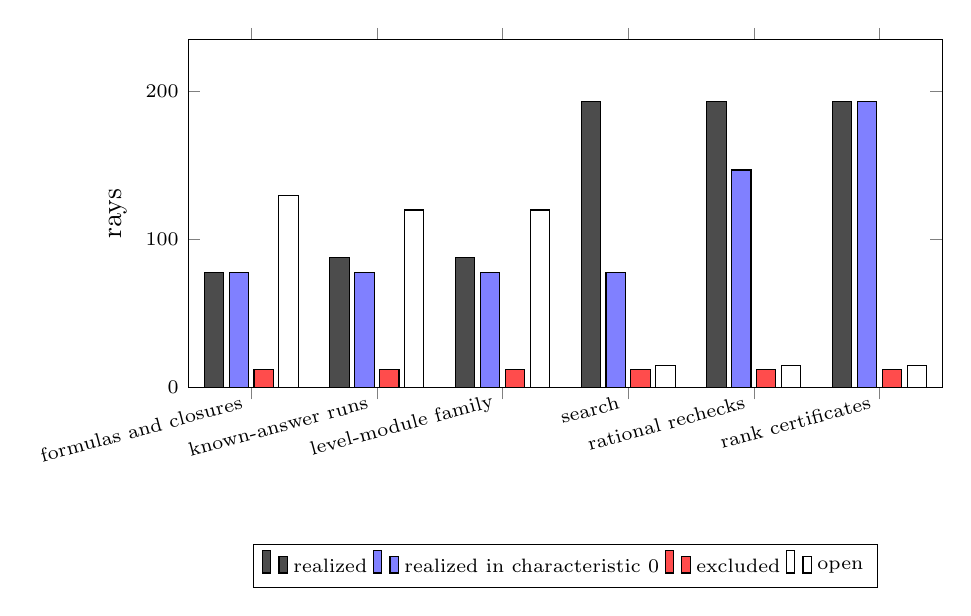
\begin{tikzpicture}
\begin{axis}[ybar, width=0.92\textwidth, height=6cm, bar width=7pt, ymin=0, ymax=235, symbolic x coords={formulas and closures,known-answer runs,level-module family,search,rational rechecks,rank certificates}, xtick=data, x tick label style={font=\scriptsize, rotate=15, anchor=east}, tick label style={font=\scriptsize}, ylabel={rays}, legend style={font=\scriptsize, at={(0.5,-0.45)}, anchor=north}, legend columns=4, enlarge x limits=0.1]
\addplot[draw=black, fill=black!70] coordinates {(formulas and closures,78) (known-answer runs,88) (level-module family,88) (search,193) (rational rechecks,193) (rank certificates,193)};
\addlegendentry{realized}
\addplot[draw=black, fill=blue!50] coordinates {(formulas and closures,78) (known-answer runs,78) (level-module family,78) (search,78) (rational rechecks,147) (rank certificates,193)};
\addlegendentry{realized in characteristic 0}
\addplot[draw=black, fill=red!70] coordinates {(formulas and closures,12) (known-answer runs,12) (level-module family,12) (search,12) (rational rechecks,12) (rank certificates,12)};
\addlegendentry{excluded}
\addplot[draw=black, fill=white] coordinates {(formulas and closures,130) (known-answer runs,120) (level-module family,120) (search,15) (rational rechecks,15) (rank certificates,15)};
\addlegendentry{open}
\end{axis}
\end{tikzpicture}
